\chapter{Software}
\label{chapter:software}

This chapter describes the implementation part of this thesis. While we do not provide any theoretical extensions to Bayesian optimization, we instead provide a modular and fully working implementation tested on multiple experiments. The implementation is provided as a Python \citep{python} package called \bopt (short for Bayesian optimization).

The main features of the package are:

\begin{itemize}
	\item A robust implementation of Bayesian optimization.
    \item Flexible experiment configuration with random search and GP backends.
    \item Parallel execution of evaluations, both on a local machine and on a cluster.
    \item Robust error handling with duplicate/similar sample detection.
    \item Command line interface for controlling experiment evaluations, including running a manual evaluation with user specified hyperparameters.
    \item Simple filesystem based storage with user-readable and editable serialization format based on YAML.
    \item Web based visualizations of the whole optimization process, including
    1D and 2D slices and marginal plots at all points during the evaluation.
    \item An ability to add manual samples either from another (already executed) experiment, or manually by running an appropriate command with user-provided hyperparameters and objective function value.
\end{itemize}


\section{Architecture}

In this section we explore the high level architecture of \bopt. Everything is structured around a central class \inlinecode{Experiment}, which represents a single objective function together with a configuration of its hyperparameters, and configuration of the Bayesian optimization itself. The \inlinecode{Experiment} can contain multiple \inlinecode{Samples}, where each sample represents a single evaluation of the objective function.

We assume the function being optimized can be evaluated by running a script file. The hyperparameters are passed as command line arguments (see \autoref{section:command-line-interface}), and the standard output of the script is parsed using a regular expression provided by the user. This provides the user with maximum flexibility with regards how the actual function is being executed, because \bopt will simply spawn the process, pass the command line arguments, and then wait for it to terminate to collect the output and parse the result. If the result is not found in the output, or the process exists with an exit code different than $0$, \bopt marks the evaluation as failed. We do not put any restrictions on the type of script the user might want to provide. It is solely at the discretion of the \inlinecode{Runner} (see \autoref{section:runners}) to figure out how to run the provided command.

Each \bopt experiment is located in its own directory on the filesystem (called the \newterm{\inlinecode{meta\_dir}}), where it stores all of the information in a single \inlinecode{meta.yml} file, along with output files for each job. This makes it easy for the user to manually inspect and edit if needed, or even backup when performing more complicated operations, such as deleting specific samples, or manually adding samples from a different experiment. Since Bayesian optimization is stateless (always starting from scratch), the user can easily combine evaluations from multiple different experiments by hand, or even delete samples which were created by an accident, such as when using manual evaluations.


\subsection{Samples, Result Collection, and Locking}

Each evaluation of the objective function is split into two parts. One being the \inlinecode{Sample}, which contains the specific hyperparameter values for $x$, kernel parameters of the GP model, which were used to compute the sample, a posterior prediction of its mean and variance, and then the second part, which is an optional \inlinecode{Job} instance, which represents the actual running evaluation. The \inlinecode{Job} simply wraps the running process with its process ID (PID) and runner-specific information on how to get its status, kill it, etc.

Every time a \bopt command is executed, or whenever a new state is required, a \emph{result collection procedure} is be called, checking the status of all running jobs, and updating their respective samples with new results or failure information. The collection procedure is performed mainly to avoid race conditions, given that the evaluations themselves are running asynchronously from the main program flow in \bopt. Apart from the collection procedure and a few exceptions, such as starting a new job, the main data structure is considered read only.

It is also worth mentioning that since multiple instances of \bopt could be running at any given time, we have employed a file locking mechanism. When the experiment directory is being accessed, a \inlinecode{.lockfile} file is created in it, and any other \bopt instance detects the lock file and waits until it is released (removed). This enables the user to use the command line utilities while an experiment is running without worrying about data corruption.

\subsection{Runners}
\label{section:runners}

Training neural networks is a computationally intensive task, and tuning hyperparameters makes it an order of magnitude more expensive. As a result, running an experiment on a local computer might not be an option. The package was designed with different evaluation environments in mind and provides a flexible concept of a \inlinecode{Runner} class, which abstracts away the procedure of starting a new evaluation, that is figuring out how and where to run the script file representing the objective function.

We provide two different runners out of the box:

\begin{description}
    \item[Local] runs the process on the same machine as \bopt.
    \item[SGE] submits a job to the Son of Grid Engine \citep{sge}.
\end{description}

All runners support job parallelism using the Constant Liar approximation (see \autoref{section:parallel-evaluations}), which is part of the reason why each \inlinecode{Sample} stores a mean prediction. This value is being used as $y$ whenever a new evaluation point needs to be chosen during parallel evaluations.

When a job is started, its stdout and stderr are redirected to a file within the \inlinecode{output} directory in the \inlinecode{meta\_dir}. The file will be named with a PID in case of a \emph{local} job, and with a job ID in case of an \emph{SGE} job. In case of the local runner we have to employ a minor trick, because when \inlinecode{popen} is being called with stdout redirection, it already requires a file handle, but at that time the process ID is unknown. We work around this problem by creating a temporary file, redirecting the output to that file, and then after \inlinecode{popen} returns a PID we rename the opened temporary file to a new name with the PID. Since UNIX systems can handle renaming of open files, this workaround causes no issues, but the behavior on Microsoft Windows is unclear. If the user needs to support Microsoft Windows, they might have to provide their own runner which does not use PIDs, but rather generates the ID based on some other procedure which makes the ID available before the child process is spawned. The SGE runner does not run into this issue, because we only specify the filename as a parameter to \inlinecode{qsub}, which then handles the process scheduling, creation, redirection, and names the output file accordingly using the new job ID.

To implement a custom runner, the user only needs to subclass two classes, namely the \inlinecode{Job} class and the \inlinecode{Runner} class. The \inlinecode{Job} class needs to mainly implement an \inlinecode{is\_finished} method (among a few other ones described in the abstract interface), which returns the status of the evaluation based on the implementation details specified in the runner. To implement the \inlinecode{Runner}, the user needs to provide a \inlinecode{start} method, which accepts the values of all hyperparameters, and returns a new \inlinecode{Job}, which will later be evaluated. An additional requirement is that a \inlinecode{Job} needs to store its result in an appropriately named file, specifically \inlinecode{job.o\$ID} in the \inlinecode{outputs} directory. We adopted this approach mainly to avoid issues with process IDs as described earlier in this section.

Lastly, it is worth mentioning that \bopt supports the UNIX \inlinecode{time} command for measuring the runtime of an evaluation. Because we allow running jobs on an SGE cluster, we can not simply take the start time and end time and subtract them to get the total run time, because the job can wait in a queue for an arbitrary amount of time.

\section{GPy}
\label{section:gpy}

Our library of choice for GP regression is the \cite{gpy2014} library, because we consider it the most stable and robust package available, and it is still being actively developed. We are mainly interested in the \inlinecode{GPy.models.GPRegression} class, which implements the regression model itself, and the \inlinecode{GPy.kern} module, which implements kernel functions. We initially used our own custom implementation of GP regression (partly shown in \autoref{section:bopt-alg}) in TensorFlow \citep{tensorflow2015-whitepaper} and SciPy \citep{scipy}, but despite the seemingly short and simple numeric algorithm for computing the regression, getting all the details right proved to be an exceedingly difficult task. Even simple numerical methods like Cholesky decomposition are often wrapped with layers of numerical stability tricks, that one does not get out of the box with libraries like NumPy \citep{numpy}.

For these reasons, we ended up utilizing the GPy library, which apart from a numerically stable implementation provides many additional benefits. Being built upon a general purpose parameter optimization library \cite{paramz}, GPy allows the user to both put arbitrary constraints on each of the parameters, as well a specify a prior distribution, which is then used when optimizing the kernel marginal likelihood.

\section{Random Search}

The core optimization loop has the ability to generate samples randomly, which is useful for two reasons. It allows creating a comparative baseline, where all the samples are generated using random search, allowing us to measure the benefits and improvements of Bayesian optimization. But it also serves to bootstrap the Bayesian optimization driven search. When choosing an initial first point of evaluation, we do not have any data to fit the model to. We could optimize the acquisition function on the prior, but since our prior has zero mean, it would simply be a uniform distribution. What we do instead is sampling each hyperparameter randomly, until we have enough data to fit the probabilistic model.

The number of random samples can increase if we are using parallel evaluations, simply because if we need to start $N$ jobs at the same time, with no prior data, we cannot even calculate a mean prediction. As a result, we start the first $N$ evaluations using random search in such case.

\section{Command Line Interface}
\label{section:command-line-interface}

Since larger experiments will be most likely executed on a computational cluster we opted for a flexible command line interface, which can be easily used over an SSH connection. The available subcommands of \bopt are:

\begin{description}
    \item[init] Creates a new experiment with a given script, configuration of hyperparameters, and runner options.
    \item[exp] Prints out the current status of the experiment, showing metadata of all evaluations.
    \item[web] Starts the web interface for evaluation visualization.
    \item[run] Starts a run loop, which tracks how many jobs are currently running, spawning new jobs as needed to fulfill the parallelism requirements, and collecting the results.
    \item[run-single] Runs a single evaluation, regardless of how many jobs are currently running.
    \item[manual-run] Runs a single evaluation with hyperparameters provided by the user. This does not utilize Bayesian optimization and simply serves as an interface to manually start requested tasks.
    \item[suggest] Prints a suggestion for the next evaluation without running it, as well as an already formatted command for \inlinecode{manual-run}, so that the user can inspect the hyperparameter values and run the command immediately if they see fit.
    \item[debug] Starts a Python debugger with the given experiment loaded in, which can be useful both for diagnosing issues as well as exploring the internal data structures.
    \item[clean] Kills all running jobs and removes all evaluations from the experiment, while keeping the initialization metadata. This command is basically just a shortcut for re-starting an experiment from scratch.
\end{description}

All commands are executed as \inlinecode{bopt COMMAND} and support the conventional \inlinecode{--help} command line argument, which prints out all available options, as well as their descriptions.

\subsection{Meta Directory, Data Corruption, and \inlinecode{-C}}
\label{section:meta-dir}

When an experiment is initialized, all of its information are stored in its own directory. This includes both the meta information about hyperparameters, run configurations and evaluations, as well as the job outputs themselves.

The \bopt command was designed such that it always tries to acquire an exclusive lock on the directory using a \inlinecode{.lockfile}, which is to prevent any race conditions and possible data corruption from running multiple instances of \bopt at the same time. Such a scenario could easily occur when the user would start a long running \inlinecode{bopt run} command, while also exploring the results, and possibly starting a few more evaluations manually using \inlinecode{bopt run-single}, \inlinecode{bopt manual-run}, or even another \inlinecode{bopt run}. Because of the locking behavior, it is completely safe to run as many instances of \bopt as needed, and the user does not need to concern themselves with causing any data corruption via the command line interface. We also make sure to always serialize the data into a new file, and then atomically move over the existing one, in order to minimize possible data corruption when the \bopt process is killed.

It is important to note that \bopt was designed with manual user intervention in mind. As such, the \inlinecode{meta.yml} file, which contains all of the experiment information, was created to be easily human editable. However, because \bopt does not use the UNIX \inlinecode{flock} mechanism (as editors do not obey it), the user has to be wary of editing the file by hand while other instances of \bopt are running. Because the \inlinecode{meta.yml} file is overwritten atomically, the user can even edit the file while \bopt is running, but they have to make sure to save at the appropriate time, e.g. not to discard the changes that were just written after the file was loaded in the editor. This problem is unlikely to occur in editors like Vim, which notifies the user of the file being changed after it was read, but it still does not prevent the user from overwriting it. If there are no existing \bopt processes running, it is completely safe to alter the \inlinecode{meta.yml} file.

All of the \bopt commands also accepts a \inlinecode{-C} command line argument, which specifies a directory to \inlinecode{cd} into before any of the main code is executed (similarly as a \inlinecode{Makefile} would behave). This behavior allows \bopt to always assume it is being executed from within the \inlinecode{meta\_dir} and simplify handling paths stored in the experiment configuration files. While this behavior is unlikely to affect the user in a negative way, it is still useful to know the semantics of the program.

We now explore two of the most important commands in more detail, \inlinecode{bopt init} and \inlinecode{bopt run}.

\subsection{The \inlinecode{bopt init} Command}

Initializing experiments is an important feature and as such the command line interface has been streamlined to allow the user to input the arguments without complicated configuration files. An example of a common \inlinecode{bopt init} call could look like the following:

\begin{center}
\begin{verbatim}
bopt init \
  --param "batch_size:int:4:128" \
  --param "gamma:logscale_float:0.5:1.0" \
  --param "lr:logscale_float:1e-6:1e-1" \
  --param "dropout:float:0.1:0.6"
  -C experiments/reinforce \
  --runner sge \
  --ard=1 --gamma-prior=1 \
  --gamma-a=1.0 --gamma-b=0.001 \
  $PWD/reinforce.sh
\end{verbatim}	
\end{center}


The first four arguments specify four different hyperparameters of the REINFORCE algorithm, namely \inlinecode{batch\_size}, \inlinecode{gamma}, \inlinecode{lr} and \inlinecode{dropout}, each with a different type and range. The general format is \inlinecode{NAME:TYPE:MIN:MAX}, where \inlinecode{NAME} can be an arbitrary name, \inlinecode{TYPE} can be one of \inlinecode{int}, \inlinecode{float}, \inlinecode{logscale\_int}, \inlinecode{logscale\_float}, and \inlinecode{discrete}, and \inlinecode{MIN:MAX} are simply the bounds of the hyperparameter. If the type of \inlinecode{discrete} is specified, instead of providing the bounds the user provides a colon separated list of possible values, which would then be encoded as ordinal integers. An example of such discrete hyperparameter could be an activation function defined as \inlinecode{activation:discrete:tanh:relu:sigmoid}. However, as mentioned in \autoref{section:architecture-search}, we do not recommend using \bopt for architecture search, which discourages from most uses of the \inlinecode{discrete} type.

The next argument \inlinecode{-C experiments/reinforce} defines the \inlinecode{meta\_dir}, where the experiment data will be stored. Next we define the runner type, which can be one of \inlinecode{local} or \inlinecode{sge}.

After the runner is defined, we configure the GP regression itself, in this case by specifying the \inlinecode{ard} flag, which allows using a separate lengthscale parameter for each component of $x$ (more details can be found in the \cite{gpy} documentation). Next we specify that we want to utilize a Gamma prior on the kernel hyperparameters, and its shape and scale parameters. A complete list of all flags for configuring the GP regression, acquisition function, kernel, and the optimizer can be found using the help flag as \inlinecode{bopt init --help}.

Lastly, we provide \bopt with the script to run, in this case it is \inlinecode{reinforce.sh}, which encapsulates our objective function. We also specify it as an absolute path using the \inlinecode{PWD} environment variable, but this is shown mainly as an interesting trick that can be useful if the \inlinecode{PATH} is not configured in the environment, where the runner will execute the job.

After the command exists, it creates a directory \inlinecode{experiments/reinforce} with a \inlinecode{meta.yml} file inside. The following listing shows the contents of the file:

\begin{center}
\begin{verbatim}
gp_config: !!python/object:bopt.gp_config.GPConfig
  acq_n_restarts: 25
  acq_xi: 0.001
  acquisition_fn: ei
  ard: true
  gamma_a: 1.0
  gamma_b: 0.001
  gamma_prior: true
  kernel: Mat52
  num_optimize_restarts: 10
  random_search_only: false
hyperparameters:
  batch_size:
    high: 128
    low: 4
    type: int
  gamma:
    high: 1.0
    low: 0.5
    type: logscale_float
  hidden_layer:
    high: 128
    low: 2
    type: int
  learning_rate:
    high: 0.1
    low: 1.0e-06
    type: logscale_float
result_regex: RESULT=(.*)
runner:
  arguments: []
  manual_arg_fnames: []
  qsub_arguments: []
  runner_type: sge_runner
  script_path: ./reinforce.sh
samples: []
\end{verbatim}
\end{center}

Apart from the command line arguments we have provided, some unspecified options were filled in with the defaults. For example, the kernel function was chosen to be the default Mat\'ern $5/2$ kernel, which was shown to perform the best on many hyperparameter tuning tasks \citep{snoek2012practical}. We have tried to make the optimization procedure as configurable as possible in case the user has any additional prior knowledge, which might help them to optimize better.

In general, there are no significant requirements on the script, which we just execute as a subprocess. We only require that it takes the hyperparameter values as command line arguments in the format of \inlinecode{--NAME=VALUE}, and outputs the objective function on its standard output. By default, \bopt parses the standard output with a regular expression \inlinecode{RESULT=(.*)}, but the user is free to specify an arbitrary value in the \inlinecode{meta.yml} file. If the user wishes to run an existing software not accepting command line arguments in this form, they have to wrap the program in a script, which pre-process the arguments given by \bopt, and pass them through in the format they require. This approach allows for maximum flexibility without having to spend large effort on building a general argument passing system. In our experiments with existing software, we only found a few cases where minor argument processing was necessary.

\subsection{The \inlinecode{bopt run} Command}

After the experiment is initialized, the user can start running evaluations. Since everything is already configured in the \inlinecode{meta.yml} file, the user only needs to run \inlinecode{bopt run -C experiments/reinforce}, or \inlinecode{cd} into the directory and execute \inlinecode{bopt run}. Both of these alternatives are equivalent.

By default, this will run $20$ evaluations in total with no parallelism. The number of evaluations can be controlled with the \inlinecode{--n\_iter} switch, while the number of jobs running in parallel is controlled by the \inlinecode{--n\_parallel} option.

To track the number of running jobs, \inlinecode{bopt run} checks the \inlinecode{meta.yml} file for the job IDs, queries status of jobs, and counts how many of them are running. This allows \inlinecode{bopt run} to correctly identify running jobs, even if the jobs were not started by \inlinecode{bopt run} itself. For example, if the user first started say $5$ evaluations by hand (e.g. using \inlinecode{bopt run-single}) and then ran \inlinecode{bopt run --n\_parallel=5} while the first $5$ jobs were still running, the instance of \inlinecode{bopt run} would correctly identify the running jobs and wait for some of them to finish before launching new ones.

\section{Visualizations}
\label{section:visualizations}

Given the complex nature of tuning hyperparameters, one might be tempted to simply run a grid search and examine the results. Ignoring the computational aspects for a moment, let us focus on the manual inspection of the results. As the number of hyperparameters grows beyond $5$ -- $10$, it becomes very difficult to infer relationships among hyperparameters from a flat list of evaluations. \autoref{figure:sample-table} shows an example of a table with $6$ different hyperparameters. To model a $6$-dimensional space, at least $15$ -- $20$ evaluations are needed to get enough information to infer relationships among the dimensions. But as the number of evaluations grow, it becomes increasingly difficult to directly infer relationships among the hyperparameters from tabular data itself.

\begin{figure}
	\begin{center}
		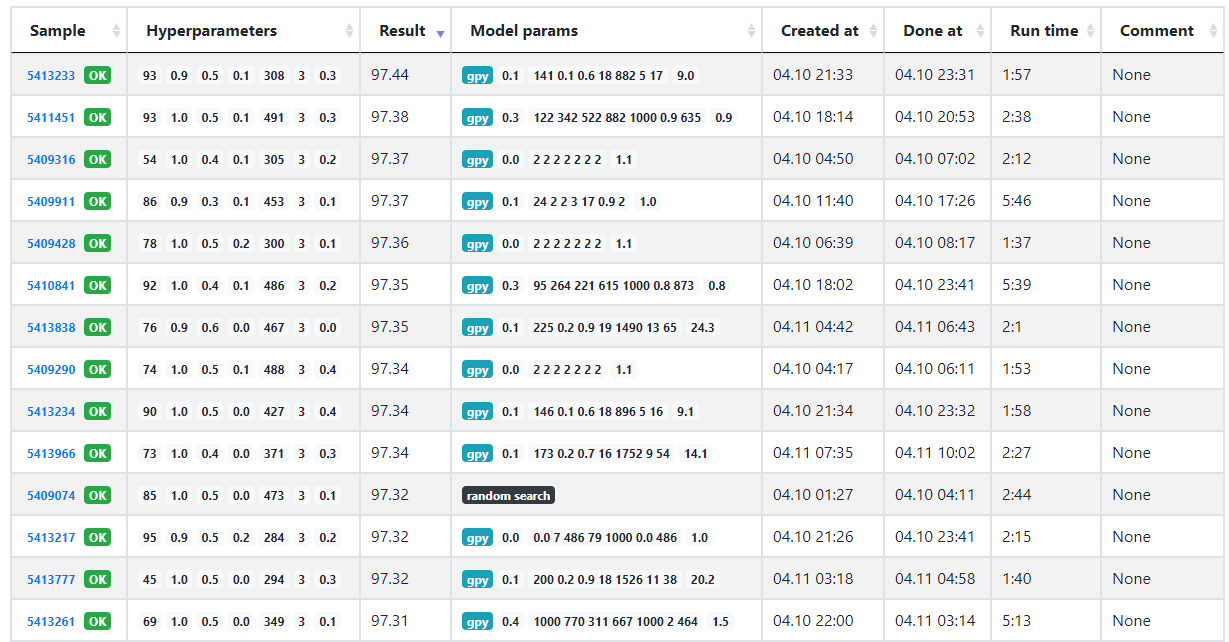
\includegraphics[width=1.0\textwidth]{images/sample-table.png}
		\caption{A table showing the results of multiple objective function evaluations.}
		\label{figure:sample-table}
	\end{center}
\end{figure}

We provide a practical solution of plotting 1D and 2D marginal GP fits for all hyperparameters and all pairs of them. In \autoref{figure:2d-marginal} we show the relationship between two of the hyperparameters as measured in one of our experiments (more details in \autoref{chapter:experiments}). We can also show each 1D marginal in order to visualize how each hyperparameter affects the fitness irrespective of the others, as shown in \autoref{figure:1d-marginal}. The 1D figures can also plot the acquisition function, which also serves as a useful debugging tool, e.g. to diagnose possible overfitting of the GP. Lastly, we allow the user to view these visualizations at any point in time during the optimization process, as shown in \autoref{figure:timeline-view}. This provides exploring the GP regression when multiple parallel evaluations were spawned.

\begin{figure}
	\begin{center}
		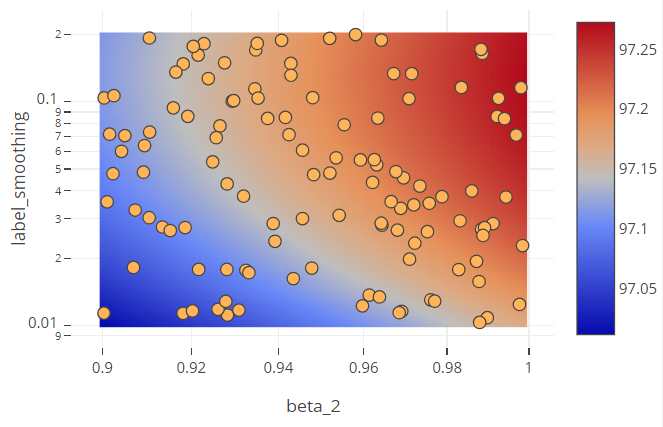
\includegraphics[width=1.0\textwidth]{images/2d-marginal.png}
		\caption{2D marginal plot showing the dependence between $\beta_2$ and \emph{label smoothing} in one of our experiments when training a larger tagger and lemmatizer network on a Czech treebank.}
		\label{figure:2d-marginal}
	\end{center}
\end{figure}

\begin{figure}
	\begin{center}
		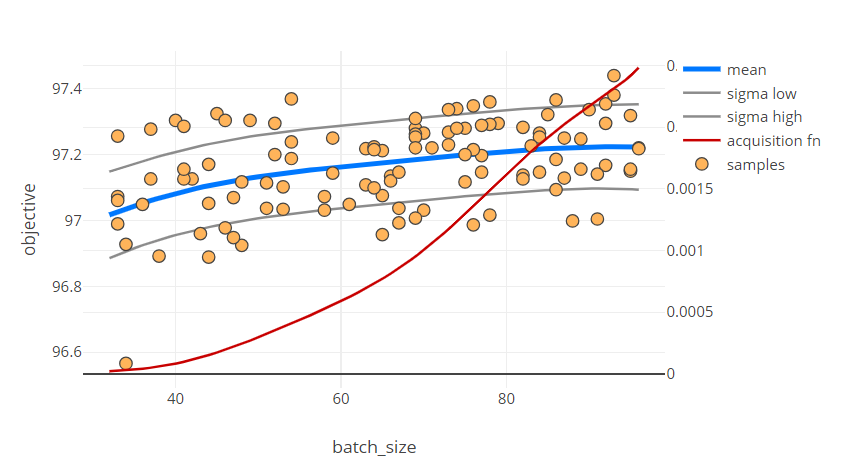
\includegraphics[width=1.0\textwidth]{images/1d-marginal.png}
		\caption{1D marginal plot showing the effect of \emph{batch size} on the objective function on the same model as shown in \autoref{figure:2d-marginal}. The red line shows the value of the acquisition function.}
		\label{figure:1d-marginal}
	\end{center}
\end{figure}

The benefit of a GP regression model is that the marginal distribution on any combination of the hyperparameters simply follows the marginalization property (see \autoref{eq:mvn-marginal-parameters}), meaning we can only consider the mean and covariance of the parameters we are interested in. All other hyperparameters get marginalized out, that is $p(\vx_2) \sim \mathcal{N}(\vx_2 | \vmu_2, \mSigma_{22})$, where $p(\vx_2) = \int p(\vx_1, \vx_2)\ d\vx_1$ and a partitioned matrix $\mSigma$ as described in \autoref{chapter:gp}. Utilizing this property, we can compute the 1D marginal projection by fitting a model to the coordinate corresponding to the hyperparameter of interest. As the goal of the marginal plots is to quickly spot trends in the data, we employ the Empirical Bayes approach described in \autoref{section:priors-on-kernel-params} to bias the prior distribution on kernel parameters towards smoother kernel functions, to avoid pathological cases of overfitting as shown in \autoref{figure:overfitting-gp}.

Similarly, we might be interested in plotting slices through the GP regression model, that is fixing a value of some hyperparameters, and examining how the objective changes when interpolating through the remaining ones. Such computation is again simple to achieve with a GP, because by slicing we are simply conditioning on the values of some elements of $\vx$, while leaving the others free. Using the conditioning formula shown in \autoref{eq:mvn-conditional-parameters}, we can compute the posterior parameters in closed form, and then simply plot the predicted mean and variance. We do not show this case in the figures since the plots look exactly the same as the marginal ones, except of course for the specific values. The user can toggle between the two modes when browsing the experiment visualisation in \bopt.

The kernel parameters for the conditioned GP are set to the exact values used when a sample was chosen for evaluation. This way we can explore the progress of the optimization process through time and inspect the state of the model at each point, understanding why it chose the hyperparameters it did.

\begin{figure}
	\begin{center}
		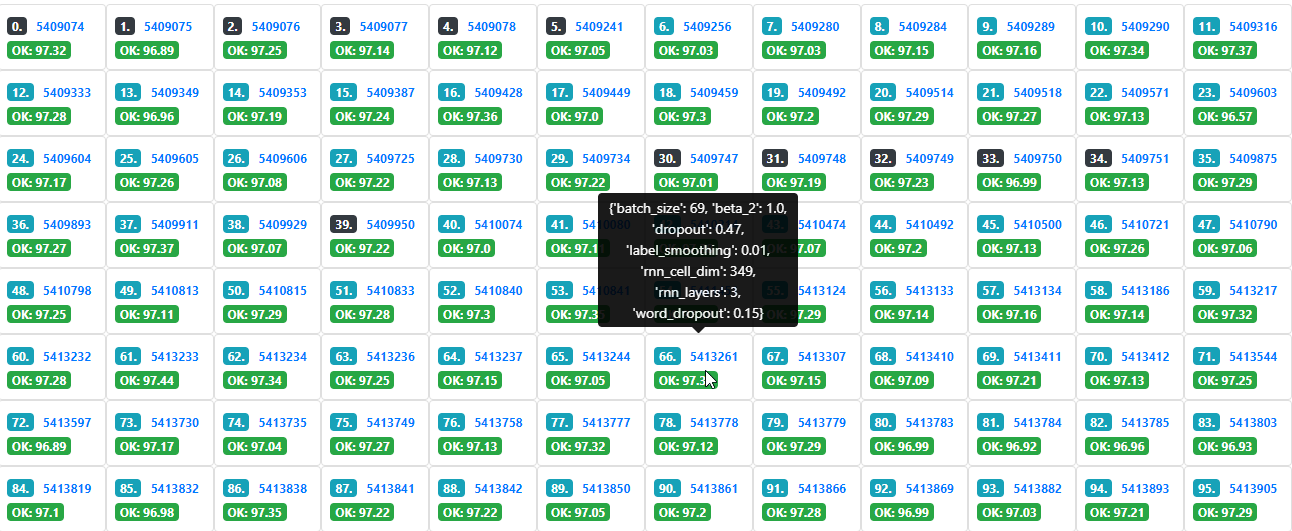
\includegraphics[width=1.0\textwidth]{images/timeline-view.png}
		\caption{A timeline showing all of the evaluated experiments, together with their objective value, model type (shown in color), and the hyperparameters used for evaluation. The user can select any of the evaluations on the timeline and all of the plots will be shown from the perspective of that evaluation, i.e. what the model \emph{saw} when choosing the hyperparameters of that specific evaluation.}
		\label{figure:timeline-view}
	\end{center}
\end{figure}


\subsection{Kernel Parameter Visualization}
\label{section:kernel-parameter-visualization}

\begin{figure}
	\begin{center}
		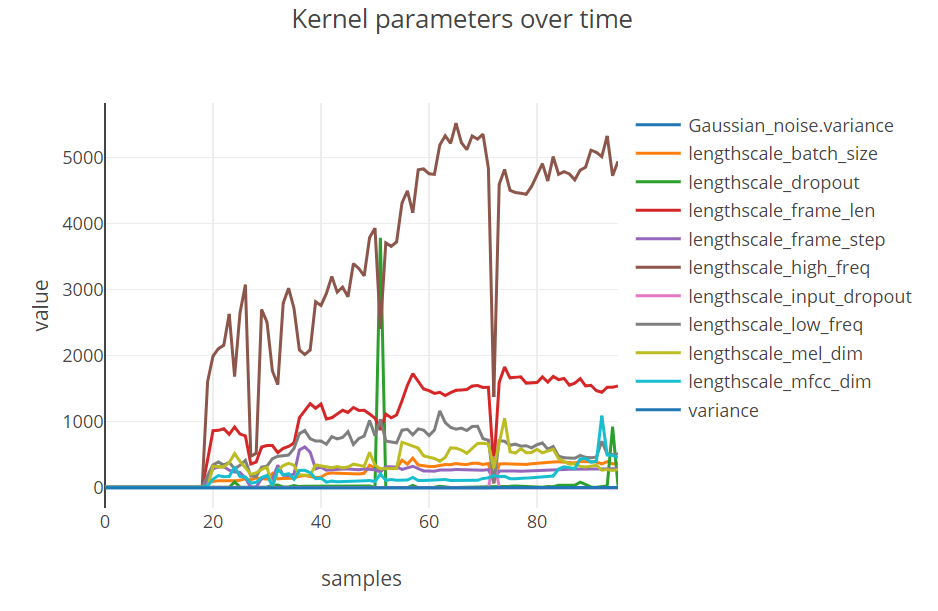
\includegraphics[width=1.0\textwidth]{images/kernel-params-over-time.png}
		\caption{Visualization of the kernel parameters over time as the Bayesian optimization progresses. In this case the model was allowed one lengthscale $\mathcal{l}$ parameter for each element of $x$, in essence allowing it to normalize each column independently. Since there are $9$ different hyperparameters, the search space is $9$-dimensional, and as a result it takes the model up to $20$ samples to find a good fit in the data. Afterwards, it automatically determines the scale of each parameter, such as the \emph{high\_freq} parameter, which was optimized on the scale of $1000$ -- $8000$. We can see the model clearly adapting its lengthscale to a similar range. As a general rule of thumb, when the lengthscale parameter is on the same order as the hyperparameter range, the model will scale that parameter to roughly unit range.}
		\label{figure:kernel-parameters-over-time}
	\end{center}
\end{figure}

\begin{figure}
	\begin{center}
		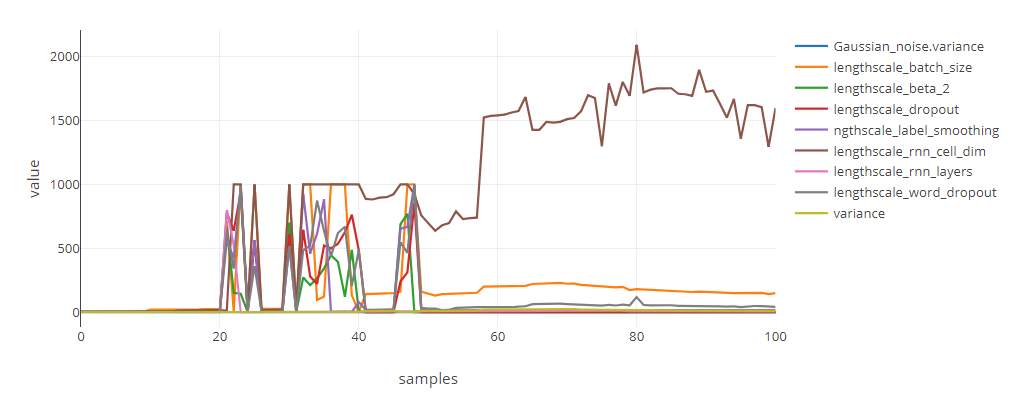
\includegraphics[width=1.0\textwidth]{images/kernel-parameters-over-time-jumpy.png}
		\caption{Visualization of a less stable model with kernel parameters rapidly changing, until around 50 samples are evaluated. In this case we attribute the instability to a very noisy objective function, where the model took a long time to fit the right value of variance to counteract the effect of the noise.}
		\label{figure:kernel-parameters-over-time-jumpy}
	\end{center}
\end{figure}

As a method of debugging possible issues in the model, as well as just general high level inspection of the quality of the fit, we provide a visualization of the kernel parameters as they change over time of the Bayesian optimization, as shown in \autoref{figure:kernel-parameters-over-time}.

The kernel hyperparameters roughly determine the general properties of the regression curve and confidence intervals. A large lengthscale results in smooth functions, while small lengthscale results in many spikes without larger continuous regions. Plotting the value of each kernel parameter as the optimization progresses allows us to judge how much does the regression model's view of the objective function change over time.

Intuitively, after we have sampled enough data points, we would expect that adding one additional sample would have an effect on the regression curve itself, but not as much on its quality, such as smoothness. A large change in the kernel parameters signifies that the objective function is now modelled substantially differently than before. We would of course expect the parameters to change over time, as the model refines itself to more data, but there should be a visible trend. In \autoref{figure:kernel-parameters-over-time} we show an example where for most of the samples the kernel parameters do not change by much, but there are two visible drops (around samples 50 and 70) in the \emph{high\_freq} lengthscale, which signify a possible issue in the GP regression at that point. Based on our experience with the model, we would still consider the example to be quite stable, compared to another example presented in \autoref{figure:kernel-parameters-over-time-jumpy}, where until around 50 samples the model was not sure how to scale individual hyperparameters, and only stabilized afterwards. In this case we attribute the problem to a much noisier model.

\subsection{Convergence}
\label{section:convergence}

Analyzing results in a table does not always explain how well is the Bayesian optimization process doing. We add a convergence plot, which shows both the intermediate values of the objective, as well as a cumulative maximum.

In some cases the model might be achieving steady increase in the objective, as shown in \autoref{figure:convergence-plot}, while in others it might fail to improve in a significant way. The following \autoref{chapter:experiments} shows experiments where even though the model showed some improvement over the baseline, it clearly did not converge as more evaluations were computed, which becomes clearly visible in its convergence plot as shown in \autoref{figure:convergence-plot-long-exp}.

\begin{figure}
	\begin{center}
		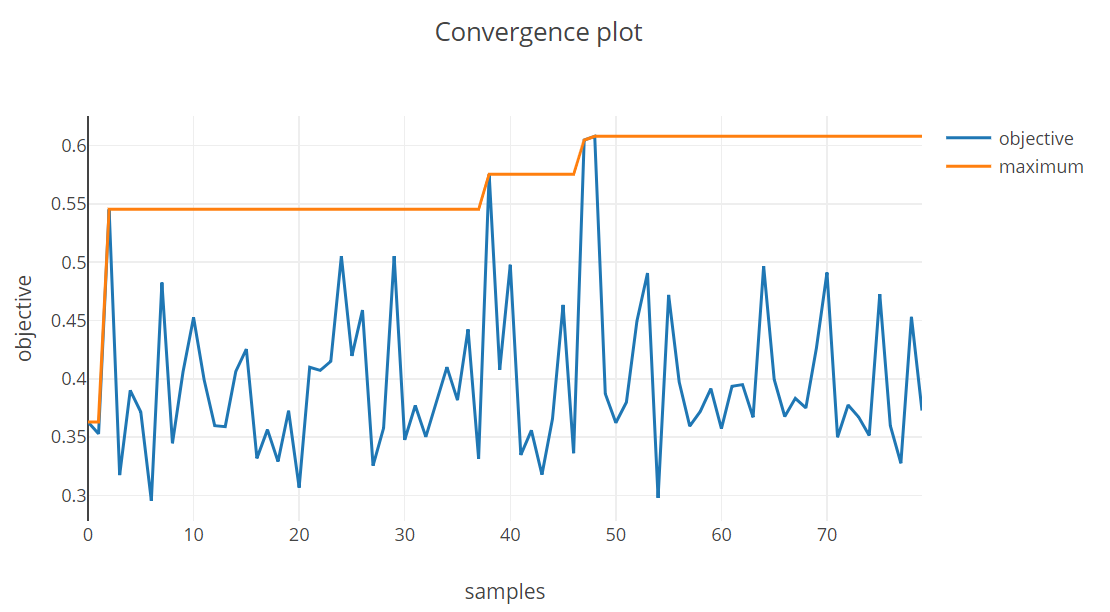
\includegraphics[width=1.0\textwidth]{images/convergence-plot.png}
		\caption{Visualization of the overall convergence of the optimization process. The $x$ axis labels time as new samples of are evaluated, and $y$ axis labels the objective function. We show both the intermediate results (blue), as well as the cumulative maximum (orange).}
		\label{figure:convergence-plot}
	\end{center}
\end{figure}

\begin{figure}
	\begin{center}
		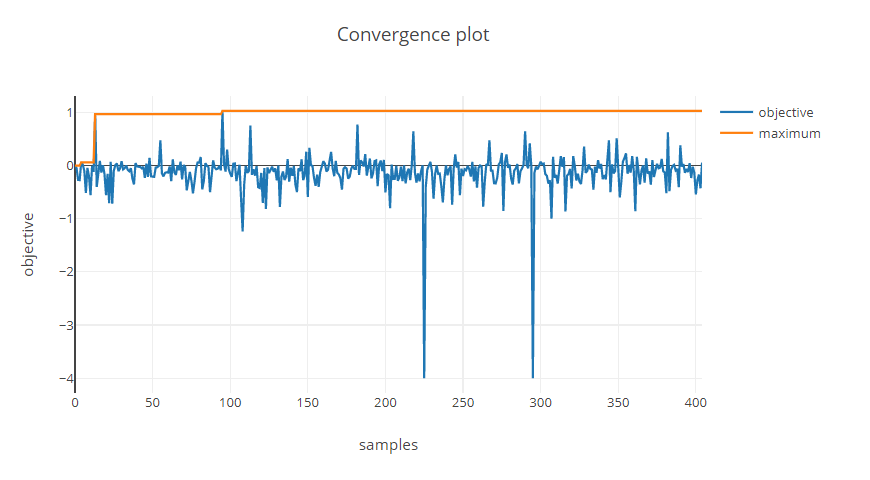
\includegraphics[width=1.0\textwidth]{images/convergence-plot-long-exp.png}
		\caption{Convergence plot of a long running experiment where no significant improvement over the baseline is found. In this particular case the objective was measured as an improvement over an existing model.}
		\label{figure:convergence-plot-long-exp}
	\end{center}
\end{figure}


\section{Inspecting Attached Experiments}

We provide results for some of the experiments as an attachment to this work. Because of the design described in \autoref{section:meta-dir}, we only need to store the \inlinecode{meta.yml} file after the results have been collected, as the collection copies all of the results from job output files to \inlinecode{meta.yml}.

Inspecting the results is then simply a matter of running either \inlinecode{bopt web -C dir} for the web interface, or \inlinecode{bopt exp -C dir} for the command line inspector, where \inlinecode{dir} is a directory containing the \inlinecode{meta.yml} file.


